% 开题报告模板:不超过一页
\documentclass[conference]{IEEEtran}

\pagestyle{plain}


\usepackage{todonotes}
\usepackage{fontspec,xltxtra,xunicode}
%\usepackage{threeparttable}
\usepackage{listings}
%\usepackage{titlesec}
%\usepackage{fontspec} % 定制字体
\usepackage{xcolor} % 定制颜色
\definecolor{mygreen}{rgb}{0,0.6,0}
\definecolor{mygray}{rgb}{0.5,0.5,0.5}
\definecolor{mymauve}{rgb}{0.58,0,0.82}
\lstset{ %
backgroundcolor=\color{white},      % choose the background color
%basicstyle=\footnotesize\ttfamily,  % size of fonts used for the code
basicstyle=\small\ttfamily,  % size of fonts used for the code
columns=fullflexible,
tabsize=2,
breaklines=true,               % automatic line breaking only at whitespace
captionpos=b,                  % sets the caption-position to bottom
commentstyle=\color{mygreen},  % comment style
escapeinside={\%*}{*)},        % if you want to add LaTeX within your code
keywordstyle=\color{blue},     % keyword style
stringstyle=\color{mymauve}\ttfamily,  % string literal style
%frame=single,
rulesepcolor=\color{red!20!green!20!blue!20},
% identifierstyle=\color{red},
%language=Java,
mathescape
}


\defaultfontfeatures{Mapping=tex-text}
%\setromanfont{Heiti} %设置中文字体
\setromanfont{SimSun} %设置中文字体

\XeTeXlinebreaklocale “zh”
\XeTeXlinebreakskip = 0pt plus 1pt minus 0.1pt %文章内中文自动换行,可以自行调节

\newfontfamily{\Song}{SimSun} %设定新的字体快捷命令
%\newfontfamily{\E}{Weibei} %设定新的字体快捷命令
\newfontfamily{\kai}{KaiTi} %设定新的字体快捷命令
\newfontfamily{\hei}{SimHei} %设定新的字体快捷命令

%\titleformat*{\section}{\hei}
%\titleformat*{\subsection}{\hei}

%%%%%% 设置字号 %%%%%%
\newcommand{\chuchuhao}{\fontsize{48pt}{\baselineskip}\selectfont}
\newcommand{\chuhao}{\fontsize{42pt}{\baselineskip}\selectfont}
\newcommand{\xiaochuhao}{\fontsize{36pt}{\baselineskip}\selectfont}
\newcommand{\yihao}{\fontsize{28pt}{\baselineskip}\selectfont}
\newcommand{\erhao}{\fontsize{21pt}{\baselineskip}\selectfont}
\newcommand{\xiaoerhao}{\fontsize{18pt}{\baselineskip}\selectfont}
\newcommand{\sanhao}{\fontsize{15.75pt}{\baselineskip}\selectfont}
\newcommand{\sihao}{\fontsize{14pt}{\baselineskip}\selectfont}
\newcommand{\xiaosihao}{\fontsize{12pt}{\baselineskip}\selectfont}
\newcommand{\dawuhao}{\fontsize{11.5pt}{\baselineskip}\selectfont}
\newcommand{\wuhao}{\fontsize{10.5pt}{\baselineskip}\selectfont}
\newcommand{\xiaowuhao}{\fontsize{9pt}{\baselineskip}\selectfont}
\newcommand{\liuhao}{\fontsize{7.875pt}{\baselineskip}\selectfont}
\newcommand{\qihao}{\fontsize{5.25pt}{\baselineskip}\selectfont}

\renewcommand\refname{参考文献}
\renewcommand{\abstractname}{{\hei 摘要}}

%%%% 下面的命令设置行间距与段落间距 %%%%
\linespread{1.2}
% \setlength{\parskip}{1ex}
\setlength{\parskip}{0.5\baselineskip}


%%% 插图, Figure --> 图
\renewcommand{\figurename}{图}
\renewcommand{\tablename}{表}


%indent
\makeatletter
\let\@afterindentfalse\@afterindenttrue
\@afterindenttrue
\makeatother
\setlength{\parindent}{2em}  %中文缩进两个汉字位


\begin{document}
%
% paper title
% can use linebreaks \\ within to get better formatting as desired
\title{2D欺骗攻击面部活性检测}


% author names and affiliations
% use a multiple column layout for up to three different
% affiliations
\author{\IEEEauthorblockN{}
\IEEEauthorblockA{孙添琦\\
tqsun@mail.ustc.edu.cn}
\and
\IEEEauthorblockN{第9组}
\IEEEauthorblockA{孙铁\\
kyles@mail.ustc.edu.cn}
\and
\IEEEauthorblockN{}
\IEEEauthorblockA{汤鑫\\
tangx@mail.ustc.edu.cn}
}

% make the title area
\maketitle

\iffalse
% 中文摘要
\begin{abstract}
论文摘要。。。
\end{abstract}

\vskip.2cm

% 中文关键词
\renewcommand{\abstractname}{{\hei 关键词}}
\begin{abstract}
关键词1;关键词2;关键词3;关键词4
\end{abstract}

\vskip.2cm

% 中图法分类号
\renewcommand{\abstractname}{{\hei 中图法分类号}}
\begin{abstract}
TP319
\end{abstract}

\vskip.2cm

% 英文摘要
\renewcommand{\abstractname}{Abstract}
\begin{abstract}
Abstract in English...
\end{abstract}

\vskip.2cm

% 英文关键词
\renewcommand{\abstractname}{Keywords}
\begin{abstract}
Keywords 1,Keywords 2,Keywords 3,Keywords 4
\end{abstract}
\fi

\section{研究背景}
当今社会人脸识别已经得到了广泛应用,然而传统的人脸识别系统往往没有考虑恶意攻击者的存在。
攻击者可以伪装成系统授权的人,从而获得对系统的非法访问。
比较典型的例子是2D欺骗攻击,它通过使用有效用户的二维面部副本来迷惑系统,是一种最常见的攻击方法。
二维欺骗攻击主要有三种类型:照片攻击、视频攻击和模拟面具攻击。
照片攻击通过在一张纸上或电子屏幕上使用合法用户的照片来逃避检测;
而视频攻击通过在电子设备上通过播放授权人员的视频来迷惑系统;
在模拟面具攻击中,对手戴着一个2D面具伪装成授权人员。

人脸活跃度检测,又称人脸欺骗检测,是为了抵御二维欺骗攻击而设计的检测手段。
人脸活跃度检测可以在人脸识别过程开始前确定图像是来自真实的还是虚假的主体。可疑图像会被过滤,而不会被传送到识别系统。

\section{研究方法}
人脸活度检测可分为基于软件和基于硬件两种方式。
以往人脸活度检测的工作主要集中在基于软件的方法上,通过分析被试的纹理、结构信息、活度标志以及所捕获图像的质量等数据来进行判别检测。
这些方法通常对环境因素敏感,比如在光照条件差、图像噪声大等情况下,检测精度会明显下降。
此外,某些活动性线索的计算复杂度较高,如基于连续帧的人脸动态计算
虽然要求用户说话或摇头可以提高检测的准确性,但由于检测时间较长且用户不一定配合,也会降低检测效率。

基于硬件的方法则是通过在识别系统中嵌入设备来获取被测试者的额外信息,比如红外检测仪器,温度检测仪器等。
虽然嵌入这些设备会让分析更为准确,但是设备安装往往较为麻烦且费用昂贵,大大增加了检测成本。

本课题拟采用基于软件的方法,通过研读相关论文研究基于软件的人脸活跃度检测并基于论文进行检测原理分析以及复现;
分别针对合法用户以及恶意用户的图像进行学习分类,对比合法用户和恶意用户的图像差异;
针对性地设计人脸信息的描述符,提取特征值,进一步通过算法增大差异并进行测试优化,以攻击者照片的通过比率来评估结果。
完成基于软件的优化之后,会继续尝试使用简单的设备嵌入进行基于硬件的活度检测,例如易于安装操作且便宜的闪光灯设备。

\section{输入数据及处理}
本次研究需要使用四种不同的检测对象:
合法用户,合法用户的照片,合法用户的视频,戴着合法用户的2D面具的攻击者。
在人脸识别检测过程中会从检测对象上获取一对图像。
\vskip.4cm
\centerline
{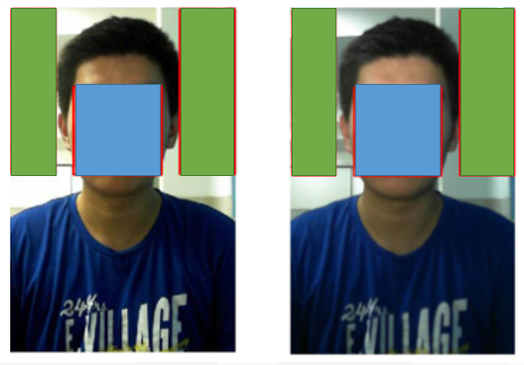
\includegraphics[width=0.33\textwidth]{p1.png}}
\centerline{\small 图1 \ \ 摄像头获取的原始待处理图像}

针对获取的原始待处理图像,主要处理三个区域:蓝色区域代表脸部区域$I_F$;
绿色区域代表背景区,为分布在左上角和右上角的两个矩形区域$I_{BR}$和$I_{BL}$。
通过对区域的处理产生对应的描述符,
例如在区域$I_F$利用基于均匀局部二值模式的描述符对人脸纹理信息进行测量,然后利用同一检测对象两张图像标准差和灰度差均值获取人脸结构信息的描述符。
不同的描述符会针对不同的攻击领域。

\vskip.4cm
\begin{thebibliography}{1}  
    \bibitem{1} D  Wen,  Han H ,  Jain A K . Face Spoof Detection With Image Distortion Analysis[J]. IEEE Transactions on Information Forensics \& Security, 2015, 10(4):746-761.
    \bibitem{2} Chan P ,  Liu W ,  Chen D , et al. Face Liveness Detection Using a Flash Against 2D Spoofing Attack[J]. IEEE Transactions on Information Forensics \& Security, 2018, 13(2):521-534.
\end{thebibliography}

\end{document}






